\chapter{Рекуррентные сети и работа с последовательностями}

Лектор: Сергей Борисович Муравьёв

\begin{remark}
    На данной лекции не будут рассматриваться способы получения эмбеддингов для текста.
\end{remark}

\section{Рекуррентные нейронные сети}

Биологические нейронные сети рекуррентны. Для поддержания аналогии с работой мозга требуется работать с рекурсивными функциями. Для них нельзя напрямую применять автоматическое дифференцирование, так как для этого требуется ациклический граф. Однако функцию можно вычислить итеративно, сводя задачу к обработке временного ряда. Временной ряд, в свою очередь, можно свести к последовательности.

\begin{remark}
    Первой реализацией такой идеи стала сеть Хопфилда, представляющая из себя реальную нейронную сеть, но тогда никто не говорил, как её обучать.
\end{remark}

Рекуррентные нейронные сети используются там, где есть последовательности
\begin{itemize}
    \item Задачи обработки и анализа текста
    \item Автоматический перевод
    \item Обработка аудио и видео:
    \begin{itemize}
        \item Прогнозирование следующего кадра
        \item Распознавание эмоций
        \item Удаление шума
    \end{itemize}
    \item Обработка изображений (например, генерация описания)
\end{itemize}

\begin{figure}[htb]
    \centering
    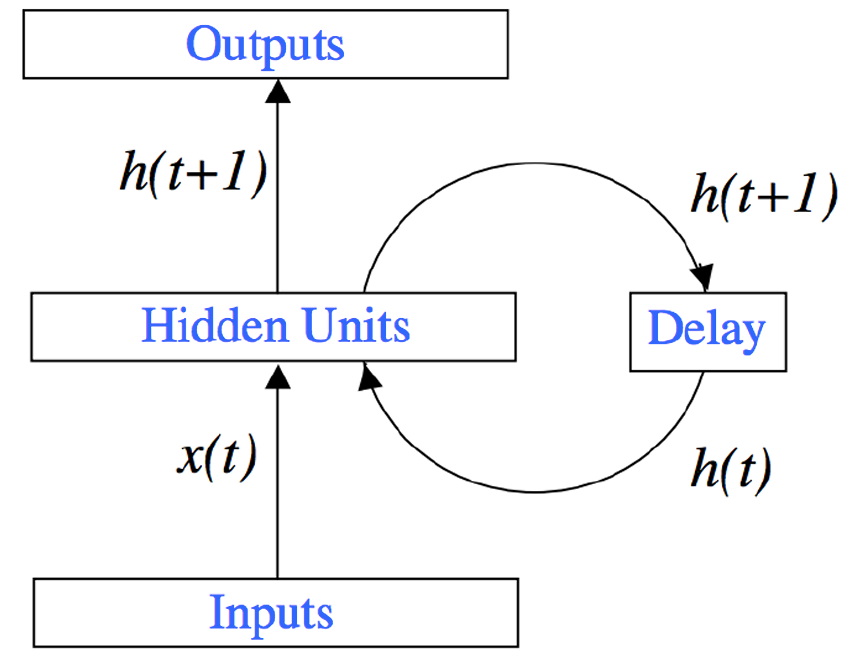
\includegraphics[scale=0.3]{images/rnn-unit.png}
    \caption{Устройство юнита рекуррентной нейронной сети}
\end{figure}

На практике обычно последовательности сводят к рекурсии, а затем обратно к последовательностям. Это полезно, например, в обработке текста, так как каждый токен в тексте связан с последовательностью предыдущих и это, конечно, необходимо учитывать. 

\begin{remark}
    Последовательность содержит "рекурсию", так как тип $Seq(X)$ можно определить рекурсивно:
    \[
        Seq(X)=\varepsilon+X\times Seq(X).
    \]
\end{remark}

\section{Обработка последовательностей}

\textbf{Области применения}:
\begin{itemize}
    \item Временные ряды
    \item Естественные языки
    \item Речь
    \item Динамические системы
    \item Изображения и видео
    \item ... 
    \item В целом, произвольные последовательности
\end{itemize}

Типы числовых последовательностей:
\begin{itemize}
    \item Спектральные
    \item Временные
    \item Частотно-временные
\end{itemize}

Временной ряд можно рассматривать как результат стохастического процесса в предположении о некоторых условных зависимостях:
\begin{itemize}
    \item Скрытые марковские модели
    \item Динамические байесовские модели
\end{itemize}

\begin{remark}
    Такие модели называются вероятностными графическими.
\end{remark}

\textbf{Преимущества RNN} (рекурентных нейронных сетей):
\begin{itemize}
    \item Могут аппроксимировать не только отдельно взятые функции, но и целые системы
    \item Являются частью "экосистемы" нейронных сетей
\end{itemize}

\textbf{Недостатки}:
\begin{itemize}
    \item Требуют очень много времени на обучение
    \item Исчезающие/взрывающиеся градиенты
    \item Всегда меняют предыдущий сигнал, который им пришел в момент времени $t-1$. Зачастую это полезно, но иногда мы не хотим его менять (однако современные архитектуры решают этот вопрос)
\end{itemize}

\section{Продвинутые архитектуры}

\begin{definition}
    \textbf{LSTM} (модуль долгой краткосрочной памяти) --- разновидность архитектуры рекуррентных нейронных сетей, предложенная в 1997 году Зеппом Хохрайтером и Юргеном Шмидхубером. Её идея состоит в том, что бы выделять отдельный блок для памяти, так как скрытые состояния плохо хранят информацию. \textbf{Блок памяти} используется в LSTM для хранения глобального состояния.
\end{definition}

\begin{figure}[htb]
    \centering
    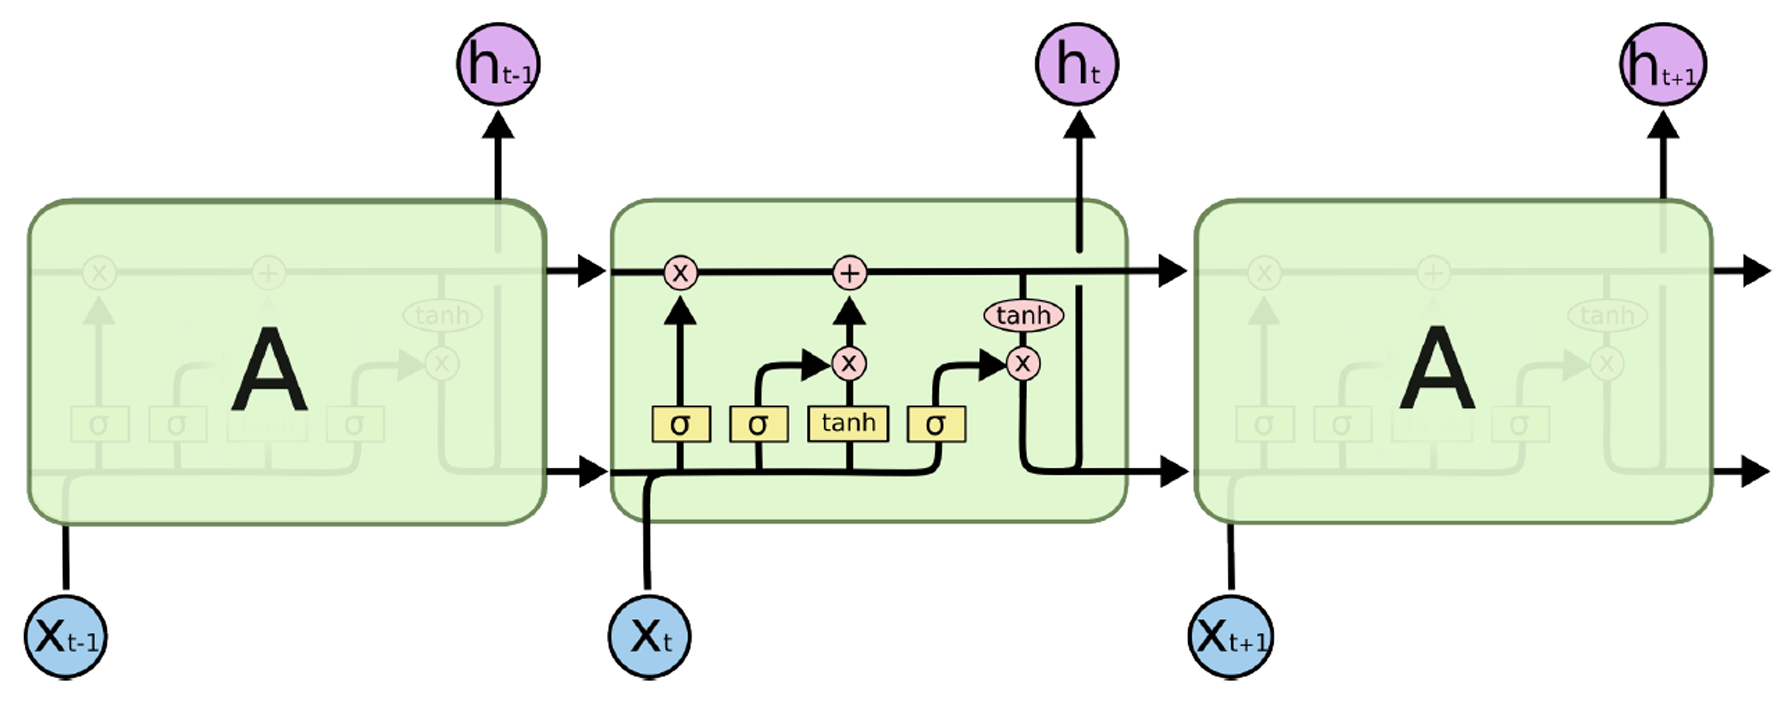
\includegraphics[scale=0.31]{images/lstm-block.png}
    \caption{Структура LSTM-блока}
\end{figure}

\begin{figure}
    \centering
    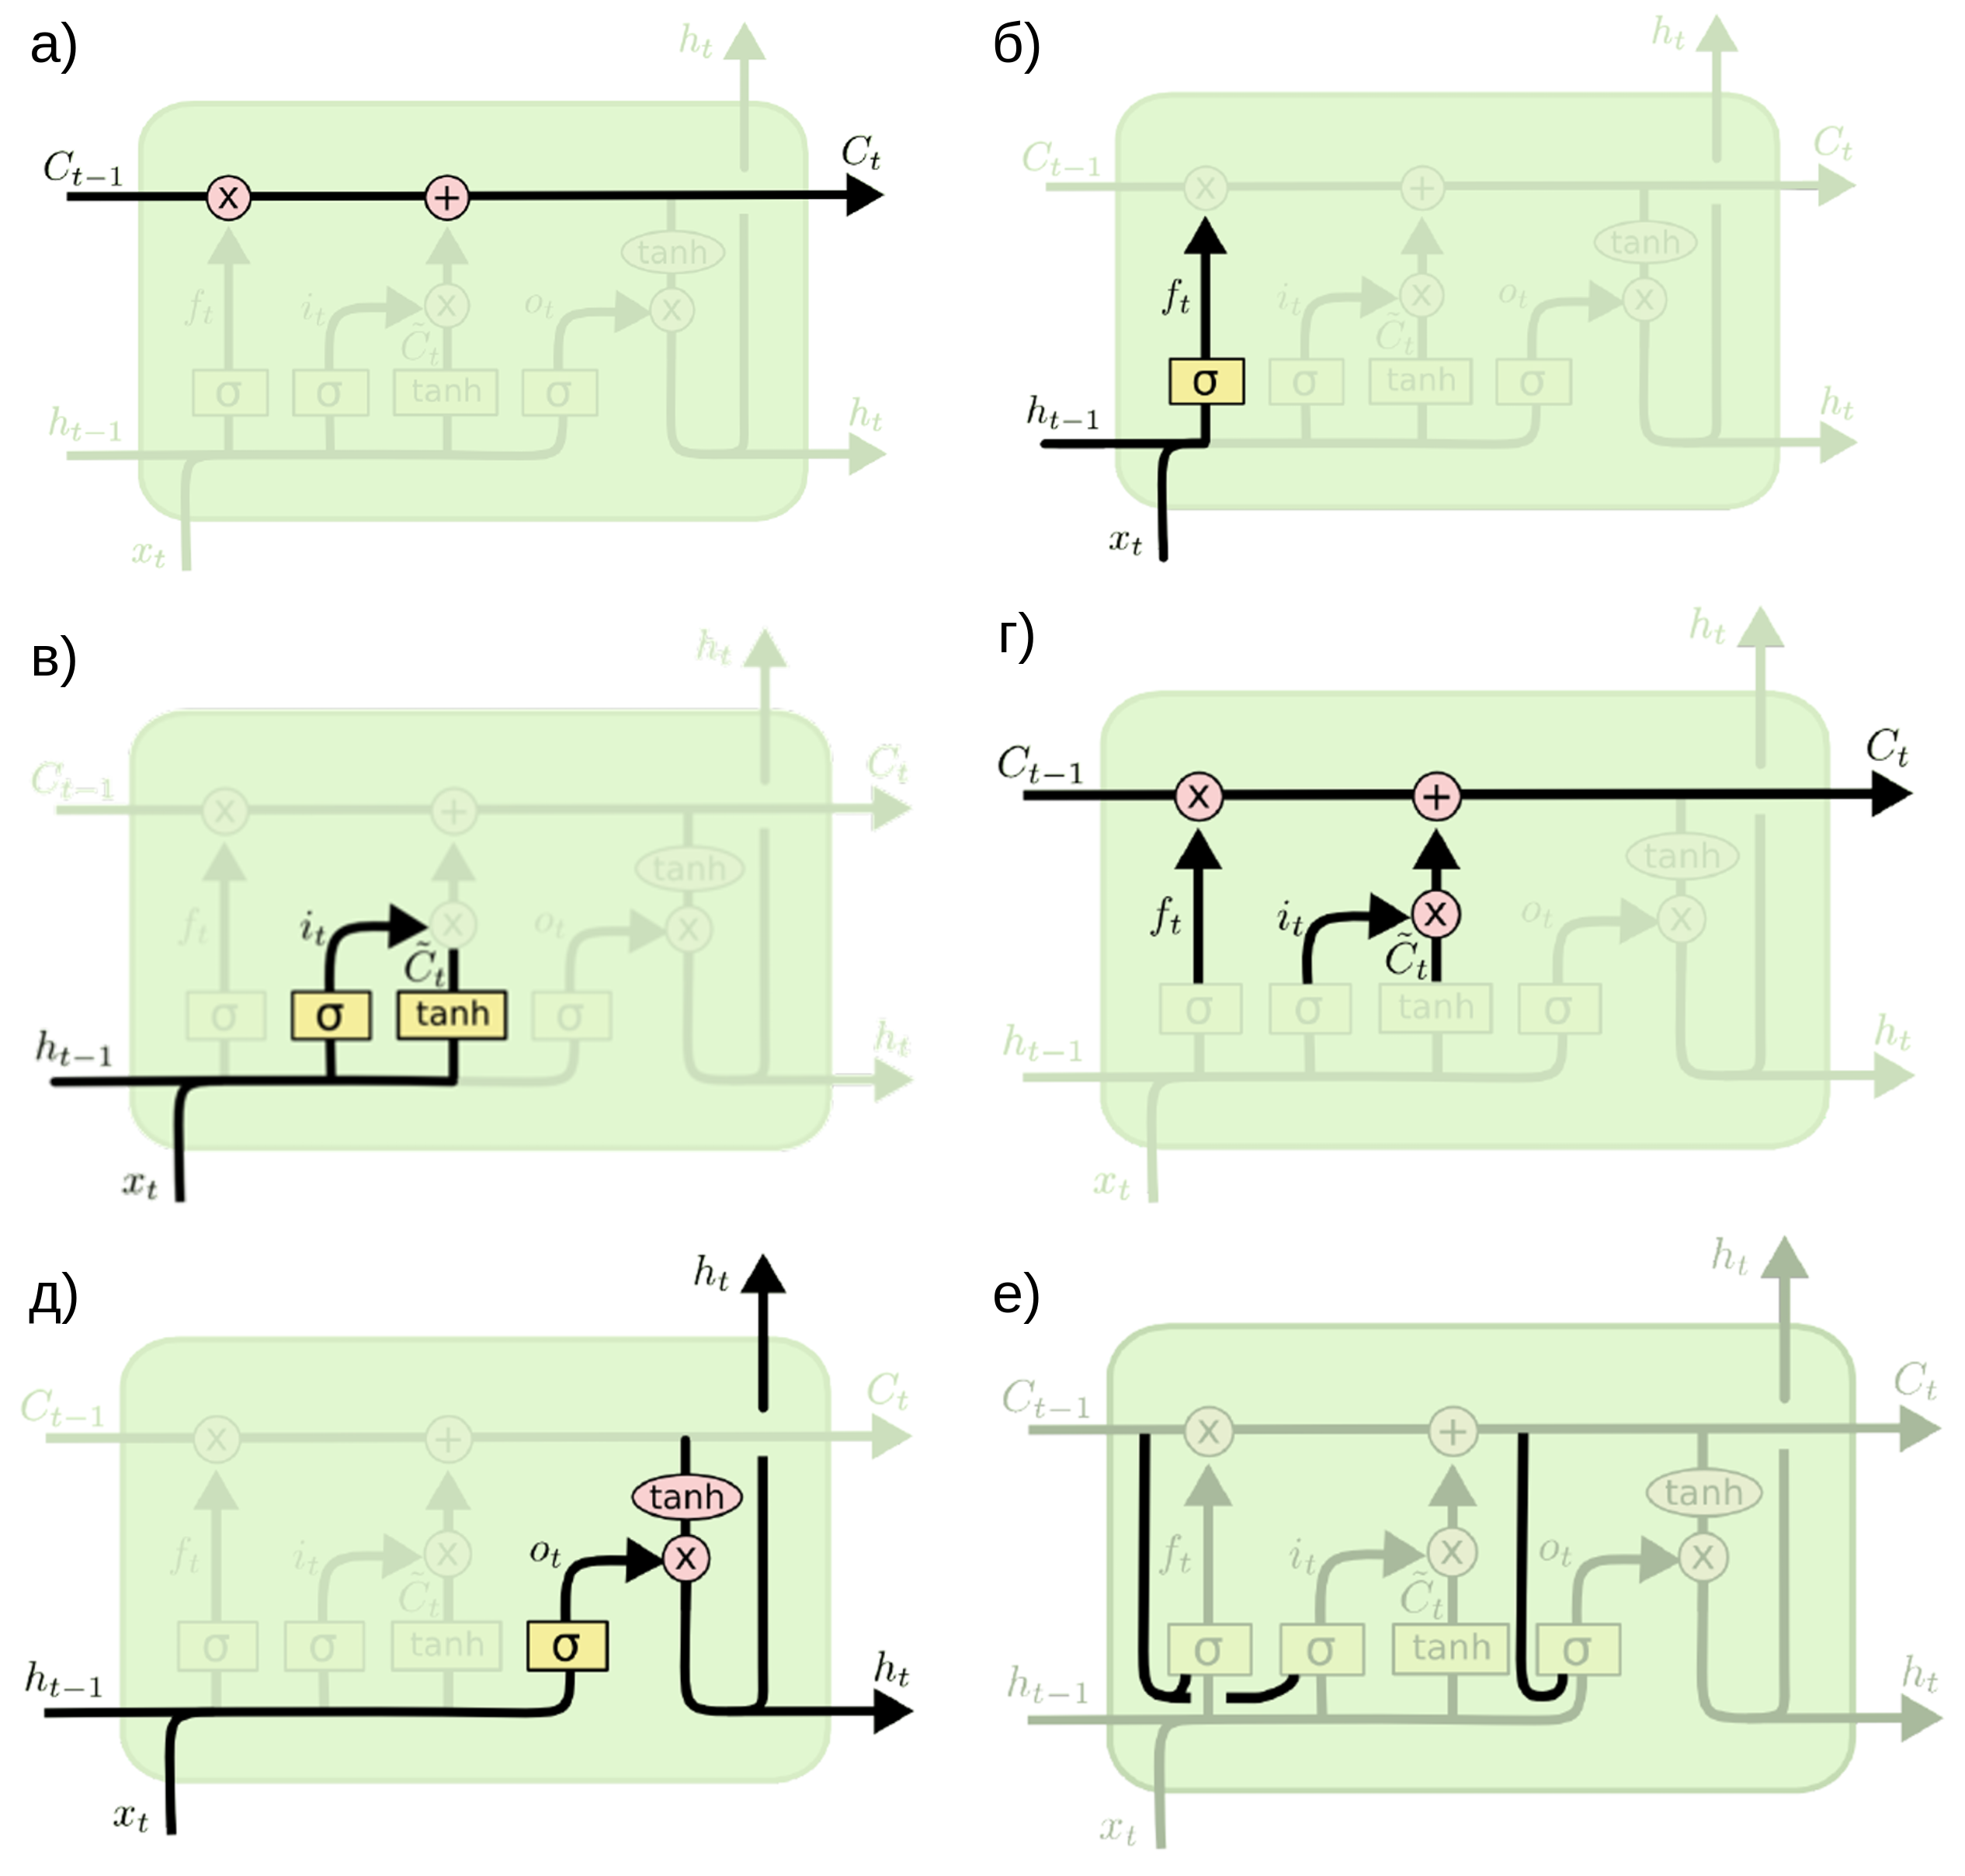
\includegraphics[scale=0.18]{images/lstm.png}
    \caption{а) Лента,  б) фильтр забывания, в) фильтр входа, г) обновление памяти, д) обновление скрытого состояния, е) LSTM со смотровыми глазками}
\end{figure}

LSTM-блок состоит из следующих компонентов (рис. 6.3):
\begin{enumerate}
    \item \textbf{Лента} (\textit{conveyor belt}) используется для накопления информации:
    \item \textbf{Фильтр забывания} (\textit{forget layer}) определяет, что нужно забыть:
    \[
        f_t=\sigma(W_f\cdot[h_{t-1},x_t]+b_f)
    \]
    \item \textbf{Фильтр входа} (\textit{input layer}) определяет, что нужно записать в память:
    \[
        i_t=\sigma(W_i\cdot[h_{t-1},x_t]+b_i)
    \]
    \[
        \widetilde{C_t}=\tanh(W_c\cdot[h_{t-1},x_t]+b_c)
    \]
    \item \textbf{Фильтр скрытого состояния} определяет, как его изменить
    \[
        o_t=\sigma(W_o\cdot[h_{t-1},x_t]+b_o)
    \]
    \[
        h_t=o_t\times\tanh C_t
    \]
    \item Опционально может содержать \textbf{смотровые глазки} (\textit{peephole connections}) память используется для обновления  себя и скрытого состояния. Тогда остальные параметры пересчитываются с учетом $C_t$:
    \[
        f_t=\sigma(W_f\cdot[C_{t-1},h_{t-1},x_t]+b_f)
    \]
    \[
        i_t=\sigma(W_i\cdot[C_{t-1},h_{t-1},x_t]+b_i)
    \]
    \[
        o_t=\sigma(W_o\cdot[C_t,h_{t-1},x_t]+b_o)
    \]
\end{enumerate}

\begin{remark}
    После вычисления фильтров забывания и входа обновляется хранимое в памяти значение:
    \[
        C_t=f_t\times C_{t-1}+i_t\times \widetilde{C_t}
    \]
\end{remark}

\begin{figure}
    \centering
    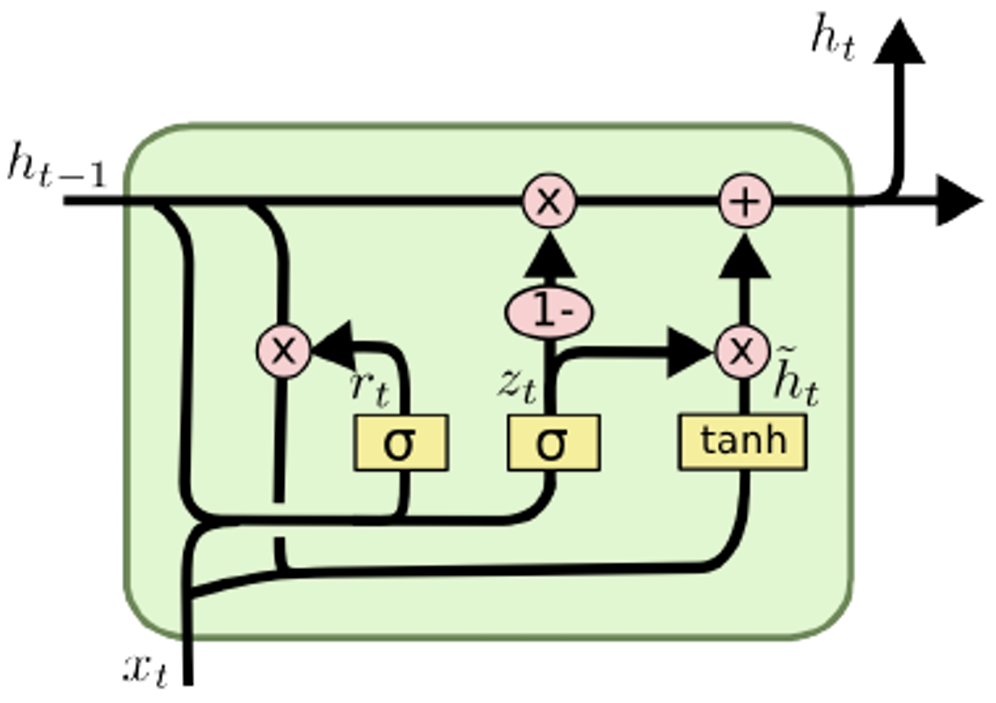
\includegraphics[scale=0.3]{images/gru.png}
    \caption{GRU}
\end{figure}

\begin{definition}
    \textbf{GRU} (\textit{gated restricted unit}) --- некоторая оптимизация LSTM, в которой меньше параметров и отсутствует выходной фильтр. Структура блока GRU представлена на рисунке 6.4. Значения в блоке пересчитываются по следующим правилам:
    \[
        z_t=\sigma(W_z\cdot[h_{t-1},x_t])
    \]
    \[
        r_t=\sigma(W_r\cdot[h_{t-1},x_t])
    \]
    \[
        \widetilde{h}_t=\tanh(W\cdot[r_t\times h_{t-1},x_t])
    \]
    \[
        h_t=(1-z_t)\times h_{t-1} + z_t\times h_t
    \]
\end{definition}

\textbf{Преимущества LSTM}:
\begin{itemize}
    \item Могут работать с удаленными во времени зависимости
    \item Нет затухания и взрыва градиент
\end{itemize}

\textbf{Недостатки}:
\begin{enumerate}
    \item Требуют много времени для обучения
    \item Всё еще забывают длинные зависимости
\end{enumerate}

\section{Больше связей}

\begin{remark}
    Иногда предыдущей информации может быть не достаточно для правильной обработки текущего сигнала. Например,\newline
    \textit{He said "Teddy bears are on sail!"}\newline
    \textit{He said "Teddy Roosevelt was a great President!"}
\end{remark}

\begin{figure}[htb]
    \centering
    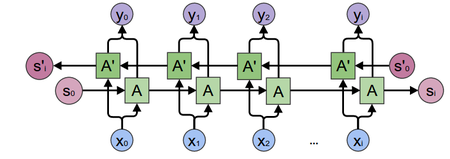
\includegraphics[scale=0.7]{images/birnn.png}
    \caption{biRNN}
\end{figure}

\begin{definition}
    \textbf{Двунаправленная RNN} (\textit{Bidirectional RNN}, \textit{biRNN}) представляет собой две однонаправленные рекуррентные сети, одна из которых обрабатывает входную последовательность в прямом порядке, а другая — в обратном. Таким образом, для каждого элемента входной последовательности считается два вектора скрытых состояний, на основе которых вычисляется выход сети. Благодаря данной архитектуре сети доступна информация о контексте как из прошлого, так и из будущего, что решает проблему однонаправленных рекуррентных сетей. Для обучения biRNN используются те же алгоритмы, что и для RNN.
\end{definition}

\begin{remark}
    На практике у biRNN всё еще есть проблемы с определением контекста.
\end{remark}

\begin{definition}
    Многослойная рекуррентная нейронная сеть --- архитектура, состоящая из нескольких слоев, каждый из которых представляет собой RNN.
\end{definition}

Классификация рекурентных нейронных сетей:
\begin{enumerate}
    \item one to one --- один вход, один выход. Примерами являются сети, которые мы обсуждали до RNN.
    \item one to many --- один вход, несколько выходов. Например, задача генерации аудио по жанру (один токен на входе)
    \item many to one --- много входов, один выход. Например, классификация тональности текста.
    \item many to many:
    \begin{enumerate}
        \item Схема перевода, выходы в которой не соотнесены со входами,
        \item Архитектура "многие ко многим", но выходы соотнесены со входами. Пример - классификация каждого слова.
    \end{enumerate}
\end{enumerate}

\begin{figure}
    \centering
    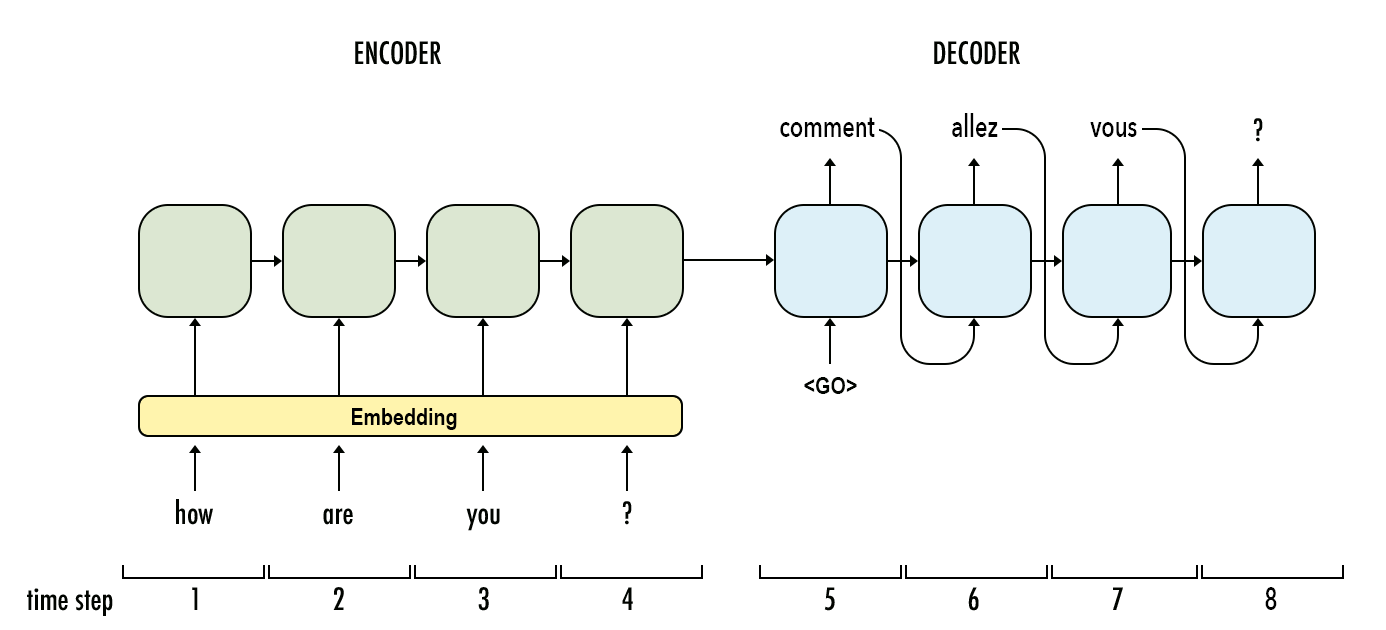
\includegraphics[scale=0.25]{images/seq2seq.png}
    \caption{Seq2Seq архитектура}
\end{figure}

\begin{definition}
    \textbf{Seq2Seq архитектура} --- архитектура, состоящая из кодировщика (encoder) и декодировщика (decoder). Получает на вход одну последовательность, возвращает другую. Ячейки в ней могут быть любой сложности. Между кодировщиком и декодировщиком передается вектор, кодирующий последовательность.
\end{definition}

\begin{remark}
    В качестве ячеек в Seq2Seq архитектуре можно использовать LSTM ячейки, а в декодировшике использовать softmax по выходу, но работает это на практике очень плохо (справедливо и для остальных рекурентных блоков):
    \begin{itemize}
        \item Кодировщик может напрочь забыть начало длинных предложений.
        \item \textit{Жадное декодирование}, когда модель пытается перевести каждое слово так, как оно есть (может решаться методом BeamSearch, когда поддерживается набор предположений - например, три наиболее вероятные гипотезы, с ними далее строится дерево, например, на пять токенов вперед и уже только потом выбирается наиболее вероятная и корректная версия).
    \end{itemize}
\end{remark}

\section{Механизм внимания}

Предложение очень сложно (невозможно) закодировать одним вектором. Поэтому для того чтобы его обработать, можно смотреть не на одно скрытое состояние, а на все скрытые состояния. Во-первых, это может частично решить проблему забывания длинных последовательностей. Во-вторых, в контексте языковых моделей это может улучшить работу с контекстом.

\begin{figure}
    \centering
    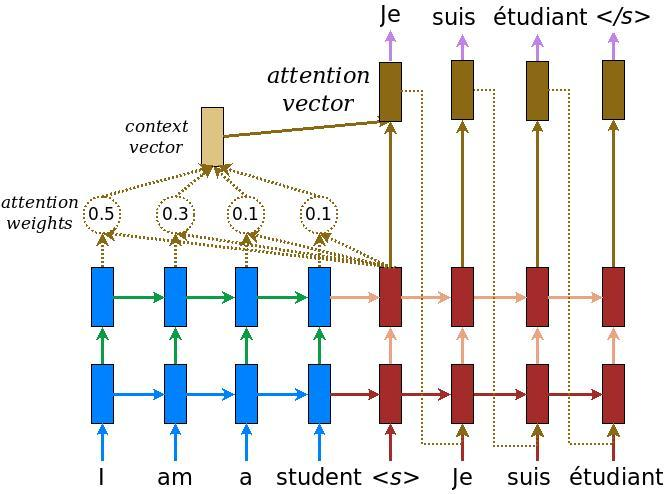
\includegraphics[scale=0.4]{images/attention-mechanism.png}
    \caption{Механизм внимания}
\end{figure}

\begin{definition}
    \textbf{Механизм внимания} (\textit{attention mechanism}, \textit{attention model}) --- техника используемая в рекуррентных нейронных сетях и свёрточных нейронных сетях для поиска взаимосвязей между различными частями входных и выходных данных.
\end{definition}

\begin{figure}
    \centering
    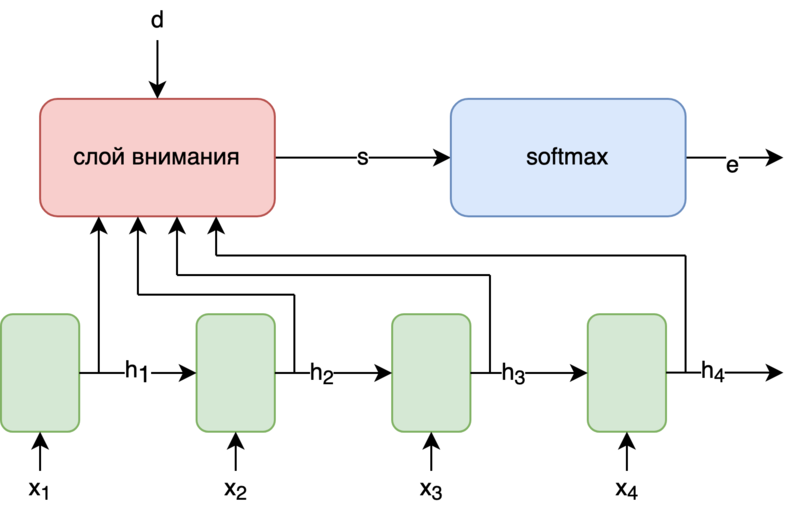
\includegraphics[scale=2]{images/rnn-attention.png}
    \caption{Обобщенный механизм внимания в RNN}
\end{figure}

\begin{figure}
    \centering
    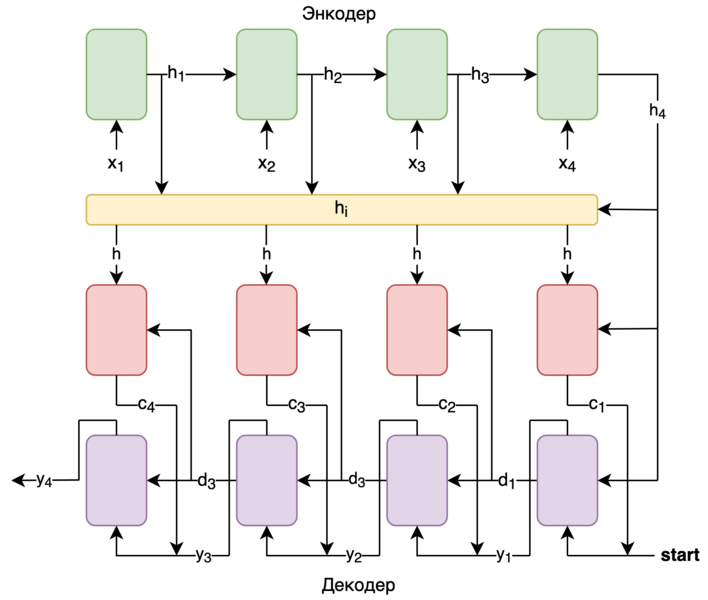
\includegraphics[scale=2.5]{images/seq2seq-attention.png}
    \caption{Пример работы Seq2Seq сети с механизмом внимания}
\end{figure}

Анализ механизма внимания:
\begin{itemize}
    \item Обучается так же, как и другие блоки
    \item Позволяет обрабатывать более длинные последовательности
    \item В целом, улучшает производительность
    \item Может применяться в произвольных сетях
    \item Добавляет больше параметров
\end{itemize}

\section{Тансформеры}

Основная идея:
\begin{itemize}
    \item Механизм внимания находит похожести между векторами.
    \item Попробуем отказаться от скрытых состояний и просто будем искать похожесть внутри входящей последовательности.
\end{itemize}

Такой подход называется \textbf{само-внимание} (\textit{self-attention}).

\begin{definition}
    \textbf{Трансформер} (\textit{transformer}) — архитектура глубоких нейронных сетей, основанная на механизме внимания без использования рекуррентных нейронных сетей. Самое большое преимущество трансформеров по сравнению с RNN заключается в их высокой эффективности в условиях параллелизации. Впервые модель трансформера была предложена в статье "Attention is All You Need" от разработчиков Google в 2017 году.
\end{definition}

Устройство трансформера состоит из кодирующего и декодирующего компонентов. На вход принимается некая последовательность, создается ее векторное представление, прибавляется вектор позиционного кодирования, после чего набор элементов без учета порядка в последовательности поступает в кодирующий компонент (параллельная обработка), а затем декодирующий компонент получает на вход часть этой последовательности и выход кодирующего. В результате получается новая выходная последовательность.

\begin{remark}
    Кодирующий компонент выглядит как стек энкодеров, а декодирующий, как стек декодеров.
\end{remark}

\begin{figure}
    \centering
    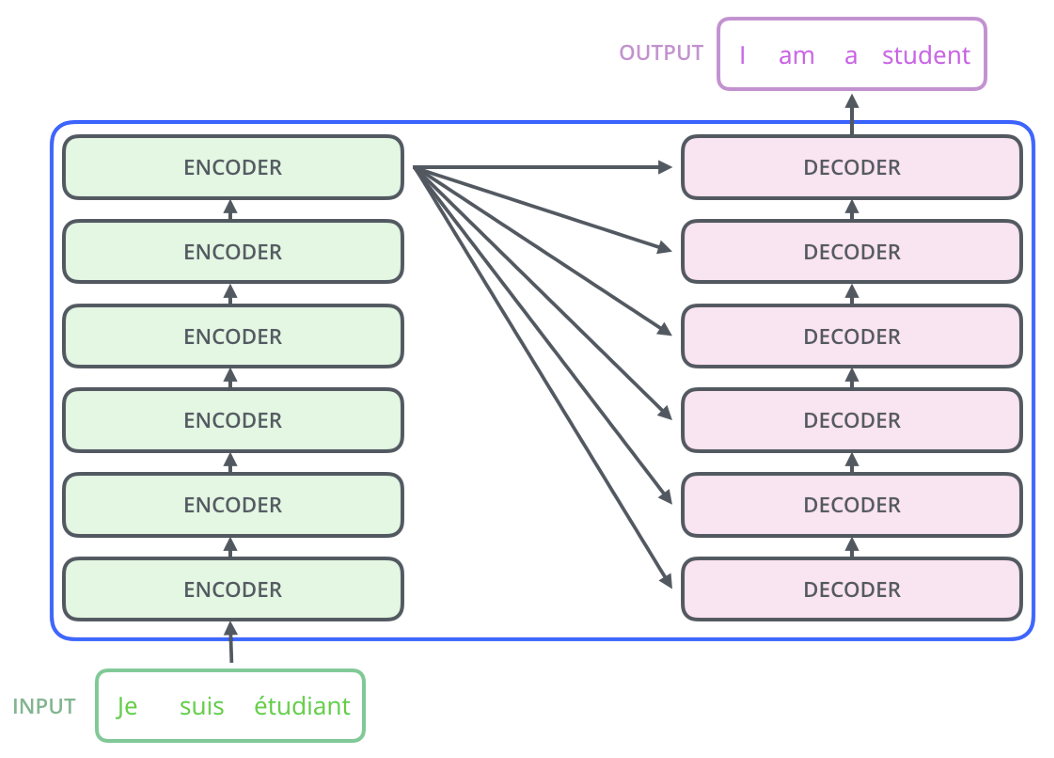
\includegraphics[scale=0.4]{images/transformer-scheme.png}
    \caption{Упрощенная схема трансформера}
\end{figure}

Строение кодировщика:
\begin{enumerate}
    \item Self-Attention
    \item Feed Forward
\end{enumerate}

Строение декодировщика:
\begin{itemize}
    \item Self-Attention
    \item \textit{Encoder-Decoder Attention} --- слой, помогающий декодировщику фокусироваться на релевантных частях последовательности
    \item Feed Forward
\end{itemize}

\begin{remark}
    Все блоки в трансформерах одинакового размера, но имеют разные параметры.
\end{remark}

Слова в трансформерах обрабатываются не последовательно, но не независимо:
\begin{enumerate}
    \item Составляется векторное представление слов (эмбеддинги)
    \item Каждое слово по отдельности проходит через два подслоя кодировщика:
        \item Они проходят через \textbf{общий} слой Self-Attention
        \item Каждое из них проходит через свой Feed Forward подслой.
\end{enumerate}

\begin{figure}
    \centering
    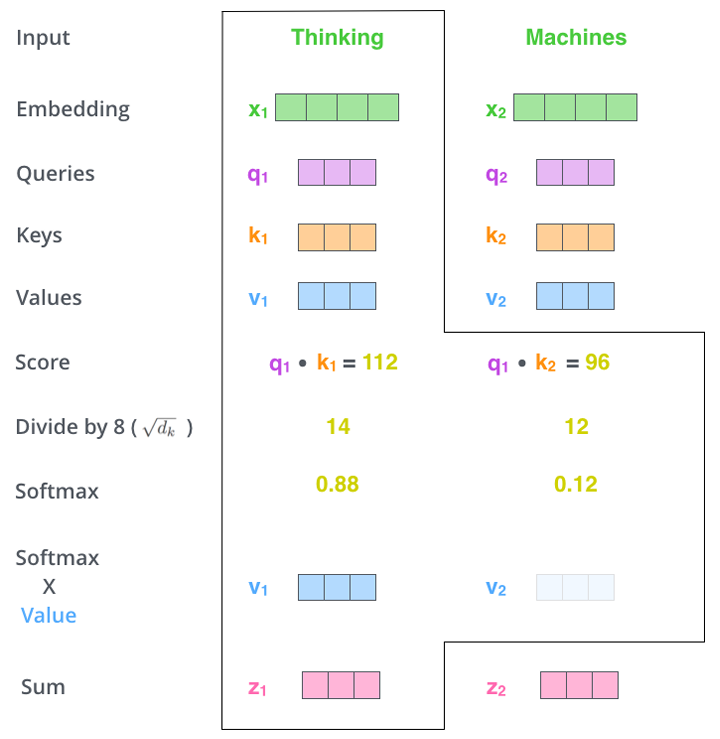
\includegraphics[scale=0.5]{images/self-attention.png}
    \caption{Механизм Self-Attention}
\end{figure}

\begin{definition}
    \textbf{Self-Attention} --- разновидность механизма внимания, задачей которой является выявление закономерности между входными данными. Для каждого вектора $x_i$ выполняются следующие действия:
    \begin{enumerate}
        \item Рассчитывается запрос (query) $q_i=Qx_i$
        \item Рассчитывается ключ (key) $k_i=Kx_i$
        \item Рассчитывается значение (value) $v_i=Vx_i$
        \item Рассчитывается score, равный $q_i\cdot k_i$
        \item Score делится на 8 (корень из длины векторов запроса, ключа и значения)
        \item Для всех слов высчитывается Softmax от значений с предыдущего шага
        \item Результат умножается на вектор $v_i$
    \end{enumerate}
\end{definition}

\begin{definition}
    \textbf{Multi-headed self-attention} — улучшенная модификация self-attention.\newline
    Слой внимания снабжается множеством «подпространств представлений» (representation subspaces). Теперь у нас есть не один, а множество наборов матриц запроса/ключа/значения. Каждый из этих наборов создается случайным образом. Далее после обучения каждый набор используется для отображения входящих векторов в разных подпространствах представлений. Также появляется способность модели фокусироваться на разных аспектах входной информации.\newline
    То есть параллельно независимо несколько раз делаем attention. Потом результат каждого attention по элементам конкатенируем, затем сжимаем получившуюся матрицу и получаем для каждого элемента свой вектор той же размерности.
\end{definition}

Дополнительные трюки, которые позволяют улучшить работу трансформеров:
\begin{itemize}
    \item \textbf{Positionsl encoding} --- способ передать модели информацию о порядке элементов последовательности путем прибавления специальных меток к вектору входных элементов. Позиции кодируются векторами $p_i$ таким образом, чтобы при увеличении $|i-j|$ увеличивался и $||p_i-p_j||$. Пример такого кодирования:
    \[
        p_{(i,s)}=
        \begin{cases}
            \sin\left(i\cdot10000^{\dfrac{-2k}{d}}\right) & \text{если }s=2k\\
            \cos\left(i\cdot10000^{\dfrac{-2k}{d}}\right) & \text{если }s=2k+1
        \end{cases}
    \]
    \item \textbf{Layer normalization}
    \item \textbf{Skip-connections}
    \item \textbf{Masked multi-head attention}
\end{itemize}

Достоинства трансформеров:
\begin{itemize}
    \item Есть возможность распараллеливания обучение модели
    \item State-of-the-art качество работы
    \item Потенциально интерпретируемые результаты
\end{itemize}

Недостатки:
\begin{itemize}
    \item Очень много параметров
    \item Нестабильно обучается
    \item Требуется фиксированная длина предложений (на текущий момент уже не так актуально)
\end{itemize}